\chapter{Metodología (Con ejemplos de figuras)}
\label{metodologia}

\section{Inserción de figuras}

Las figuras son un caso un poco especial ya que \LaTeX~busca el mejor lugar para ponerlas, no siendo necesariamente el lugar donde está la referencia. Por ello es importante añadirle un ``caption'' y un ``label'' para poder hacer referencia a ellas en el párrafo correspondiente. Nosotros ponemos la referencia a la figura \ref{multiimagen} que está en la página \pageref{multiimagen}, justo aquí debajo, pero \LaTeX ~puede que la ubique en otro lugar. (observa el código \LaTeX~ de este párrafo para observar como se realizan las referencias. Estos detalles también se aplican a tablas y otros objetos).

\begin{table}[h]
\centering
\begin{tabular}{ccc}
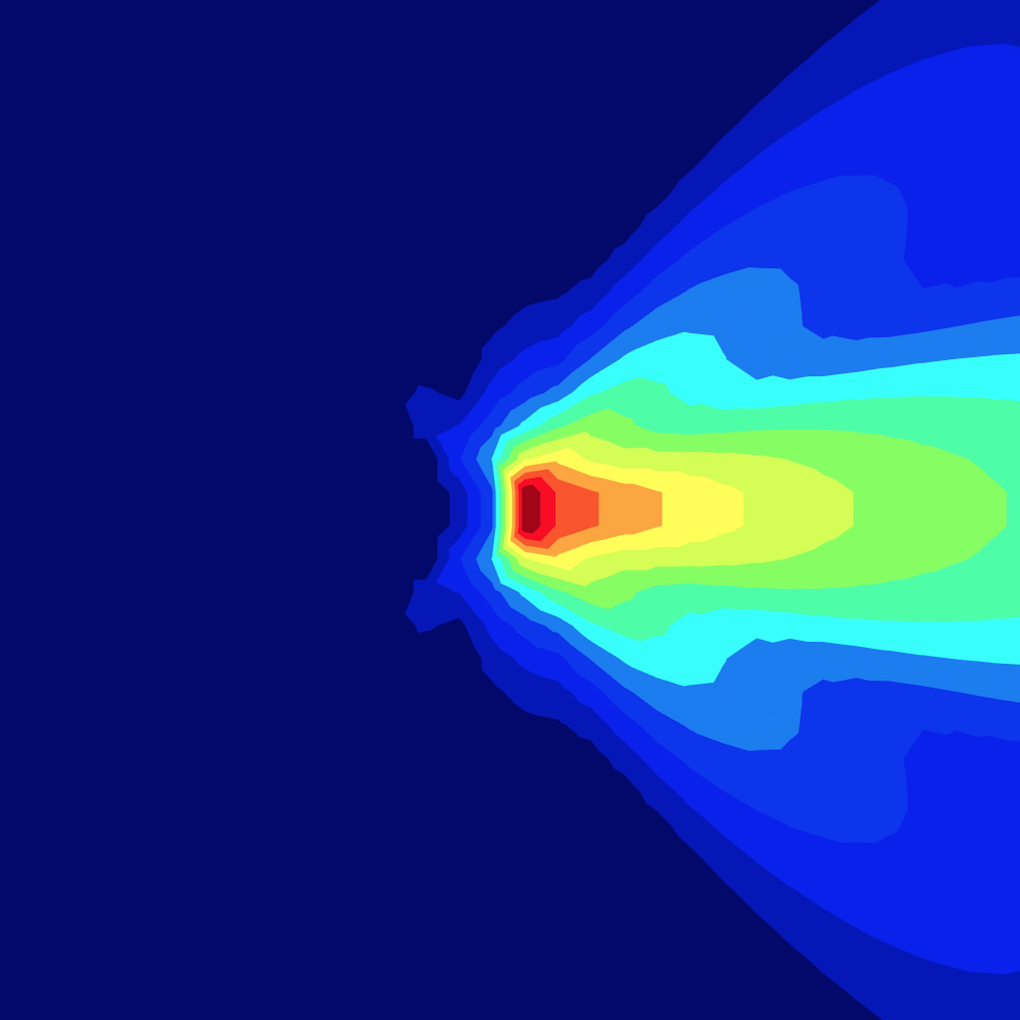
\includegraphics[scale=0.2]{archivos/130} & 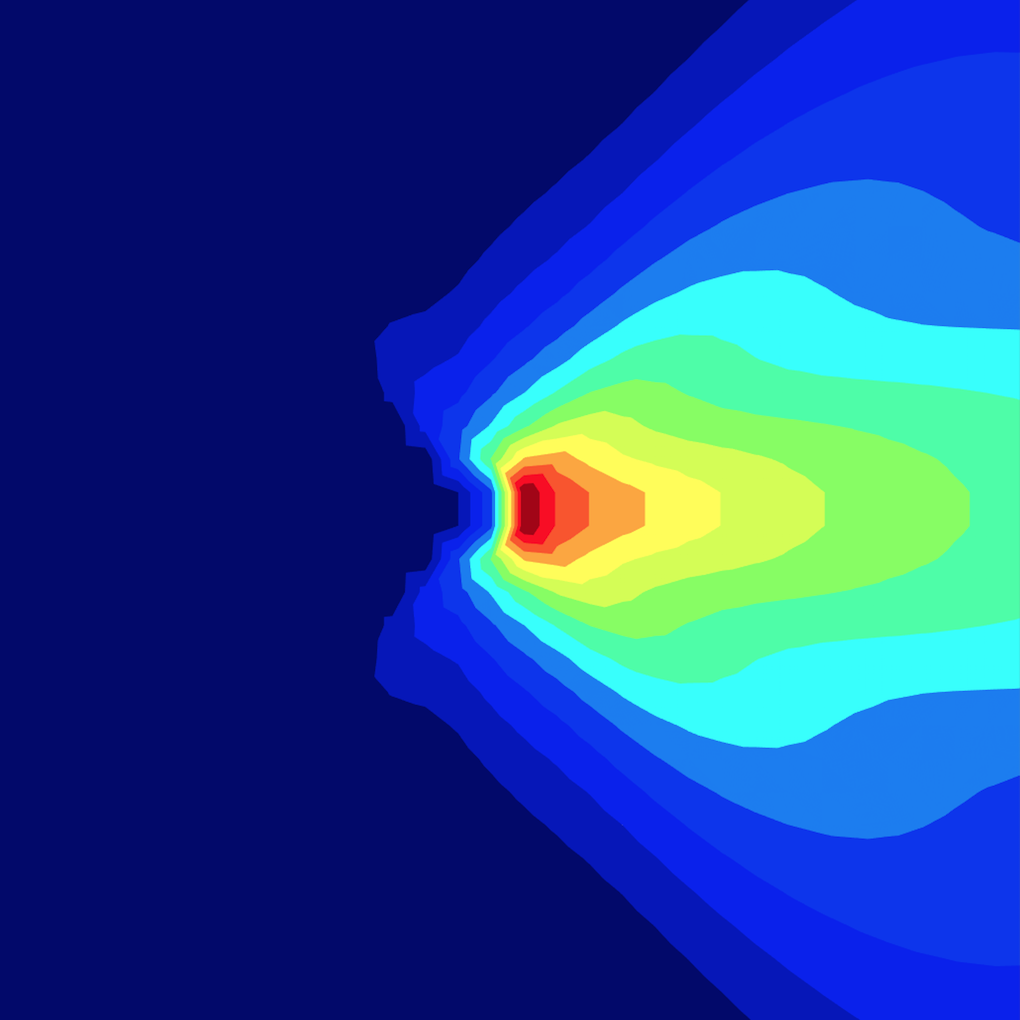
\includegraphics[scale=0.2]{archivos/160} & 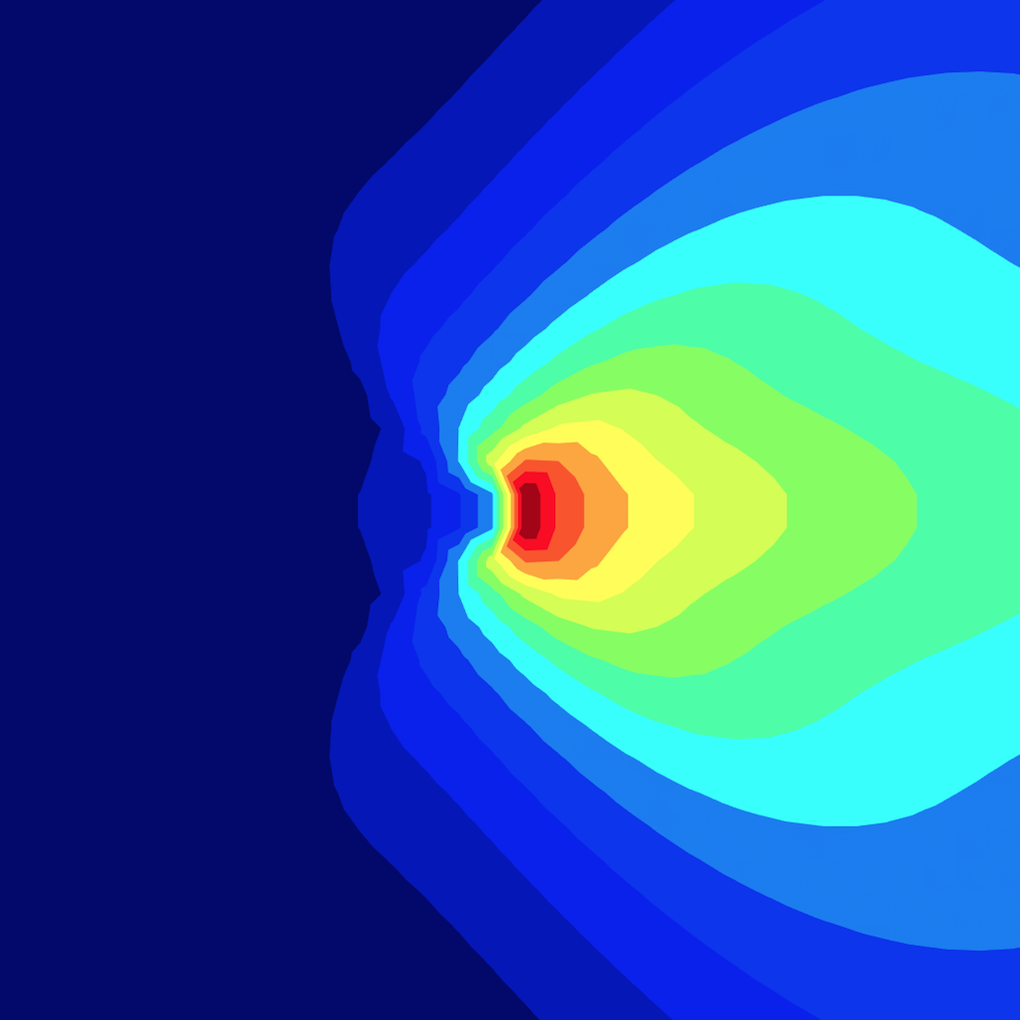
\includegraphics[scale=0.2]{archivos/190} \\
$Dist=1m \; ; \; \phi=30º$  & $Dist=1m \; ; \; \phi=60º$  & $Dist=1m \; ; \; \phi=90º$  \\
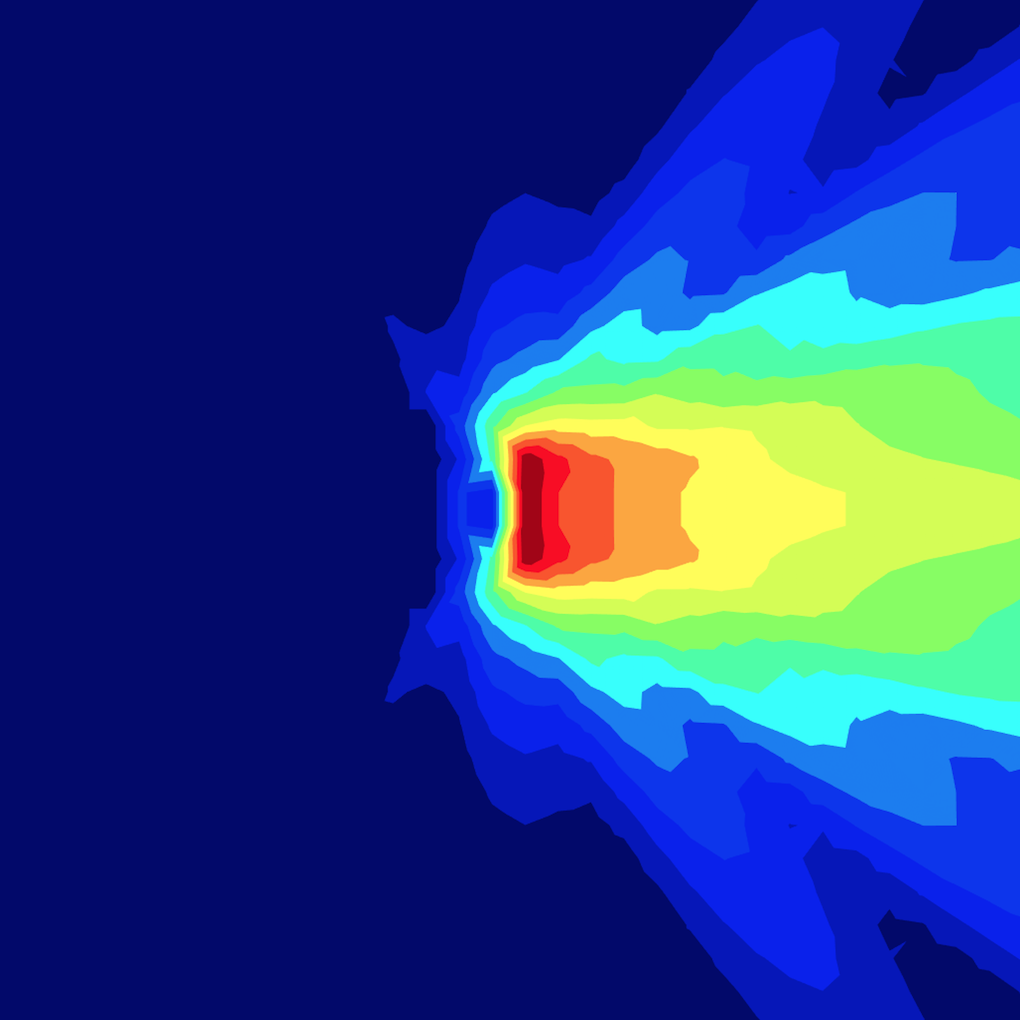
\includegraphics[scale=0.2]{archivos/230} & 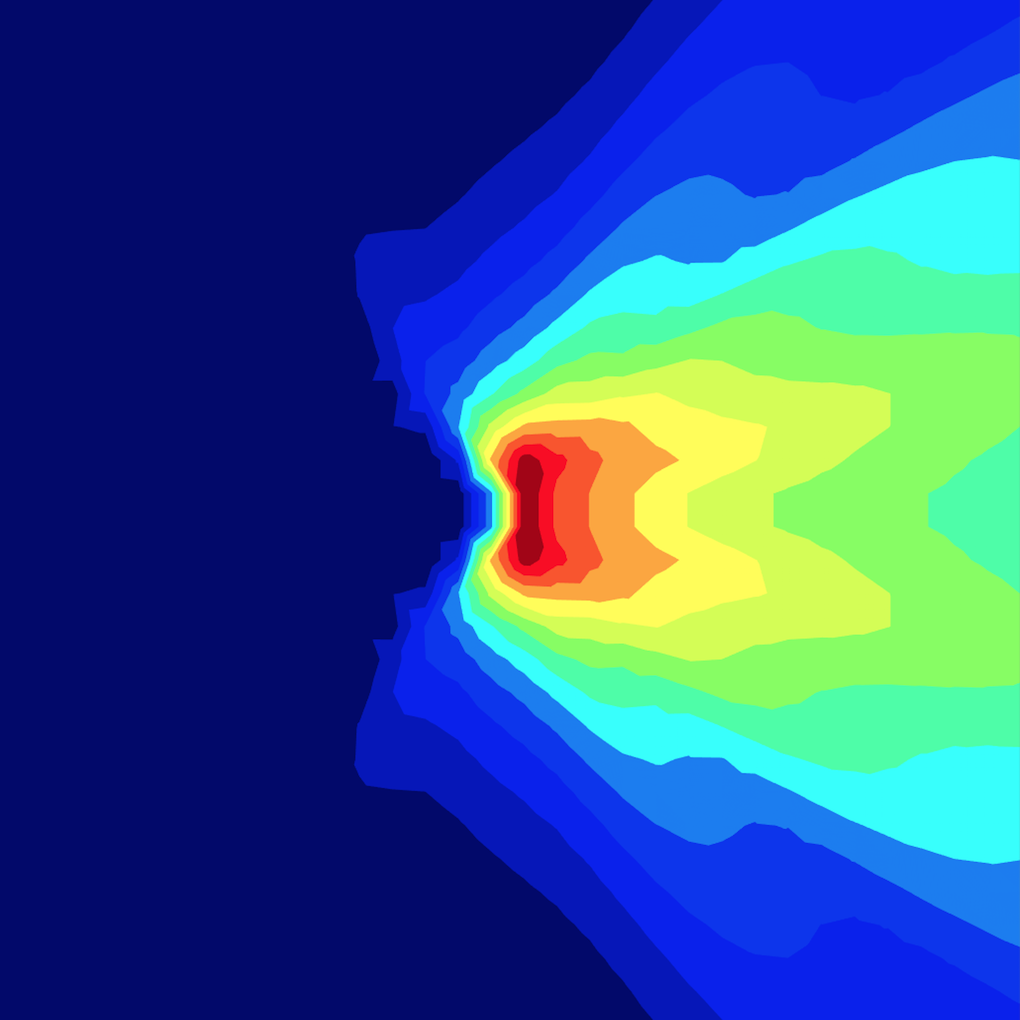
\includegraphics[scale=0.2]{archivos/260} & 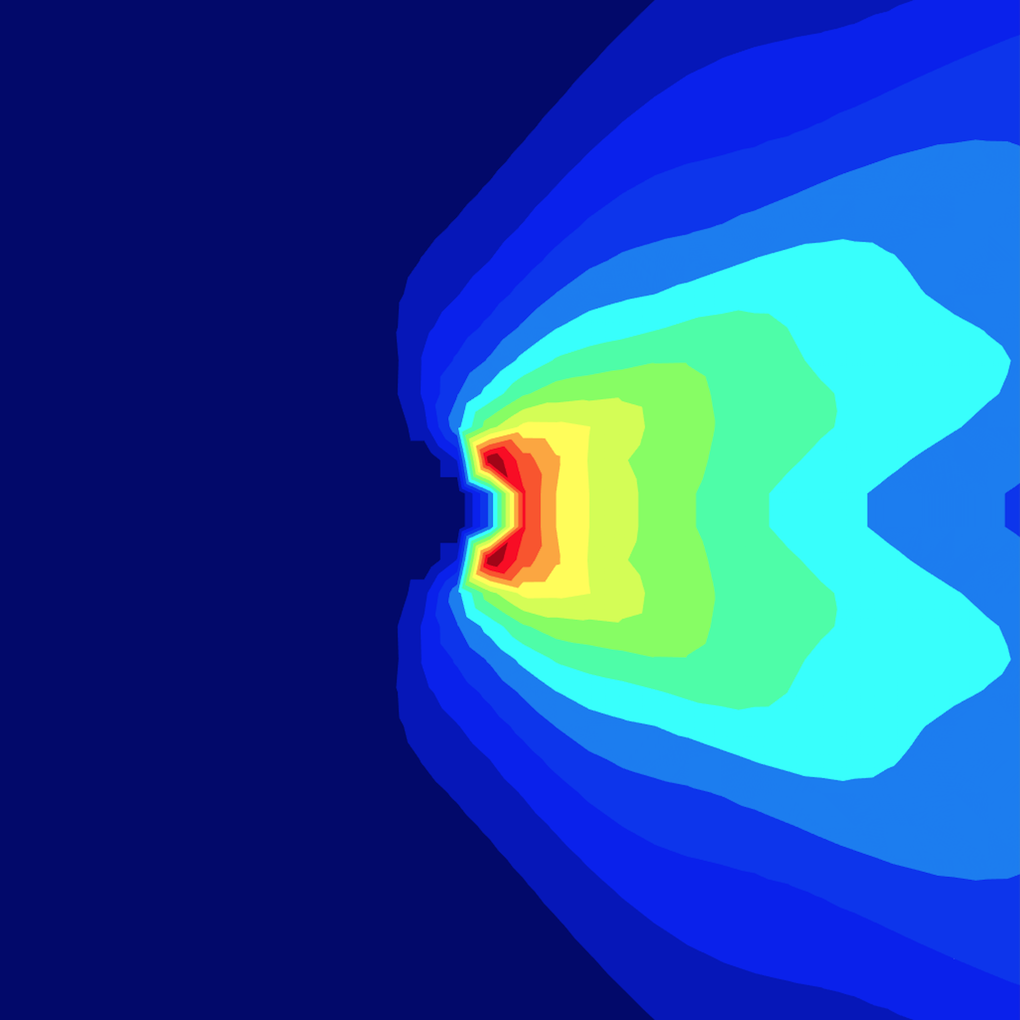
\includegraphics[scale=0.2]{archivos/290} \\
$Dist=2m \; ; \; \phi=30º$  & $Dist=2m \; ; \; \phi=60º$  & $Dist=2m \; ; \; \phi=90º$  \\
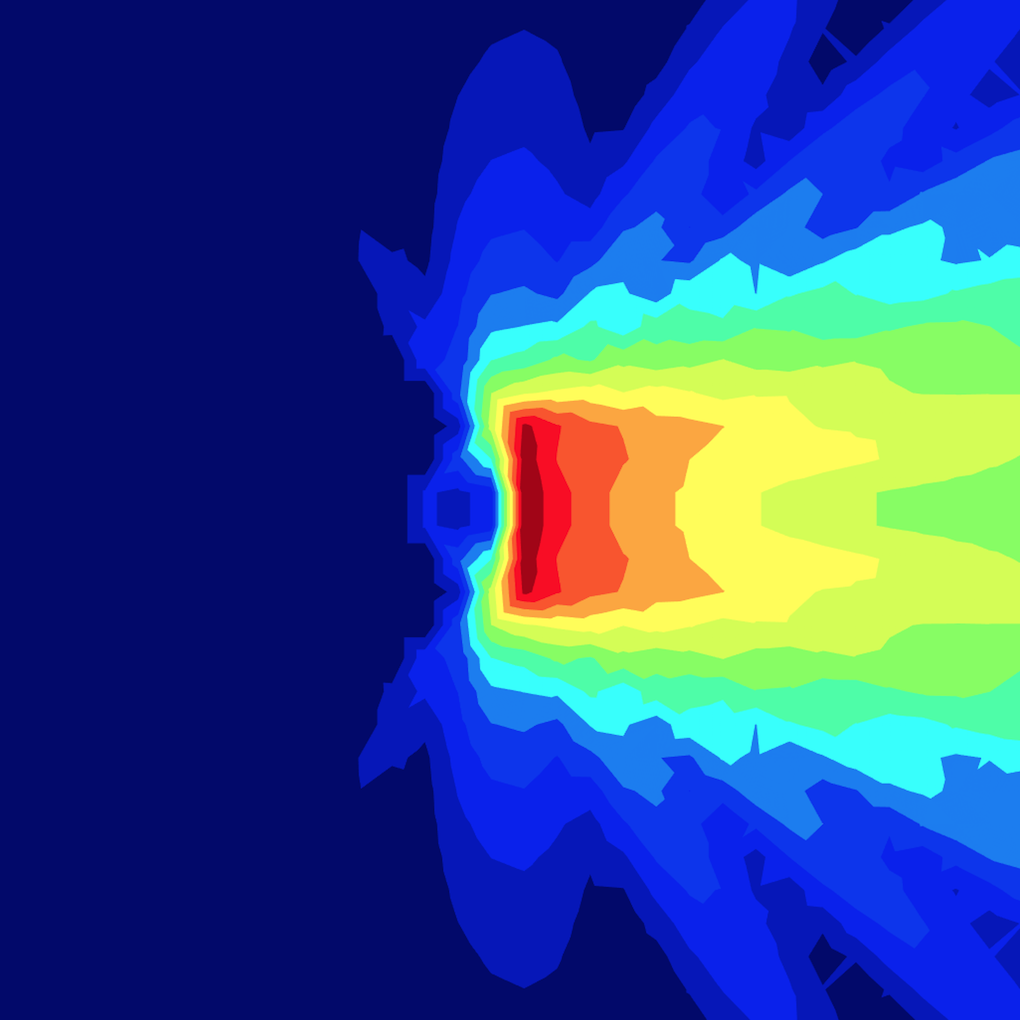
\includegraphics[scale=0.2]{archivos/330} & 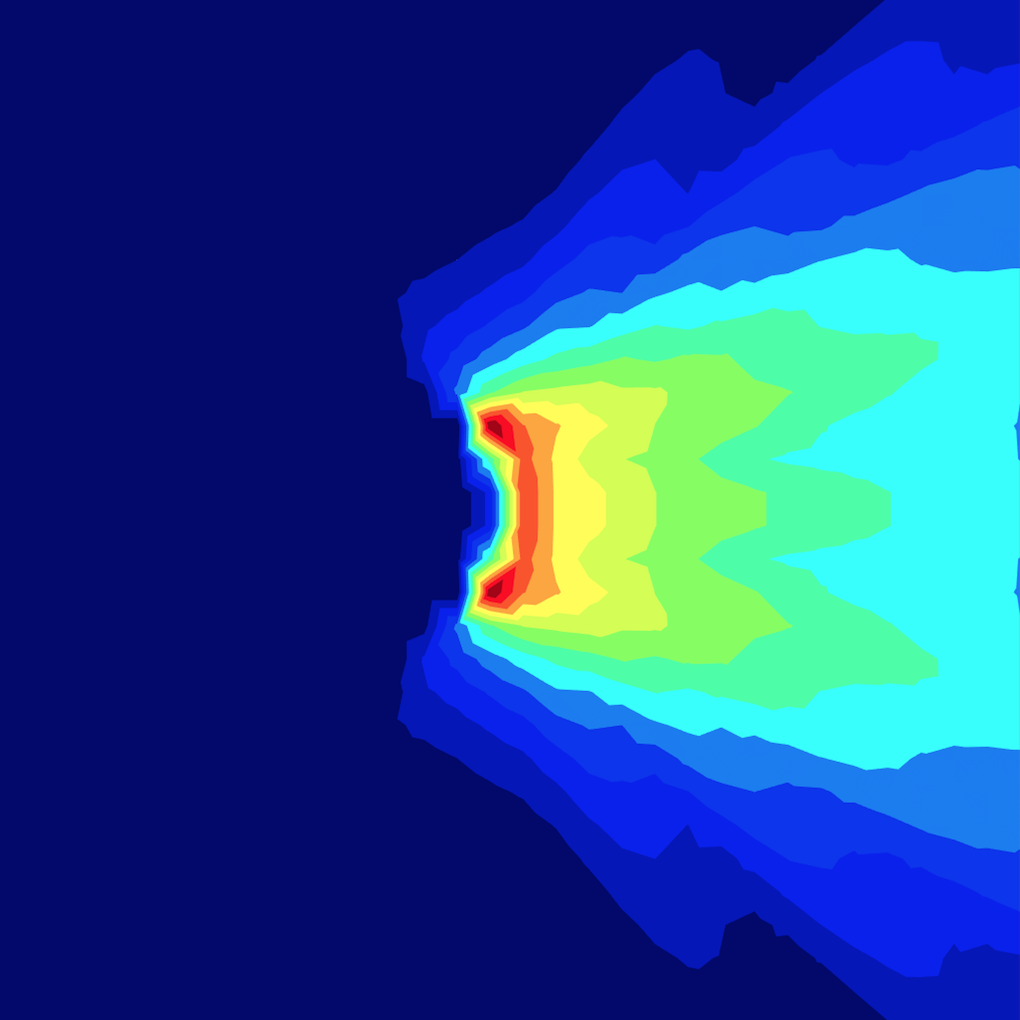
\includegraphics[scale=0.2]{archivos/360} & 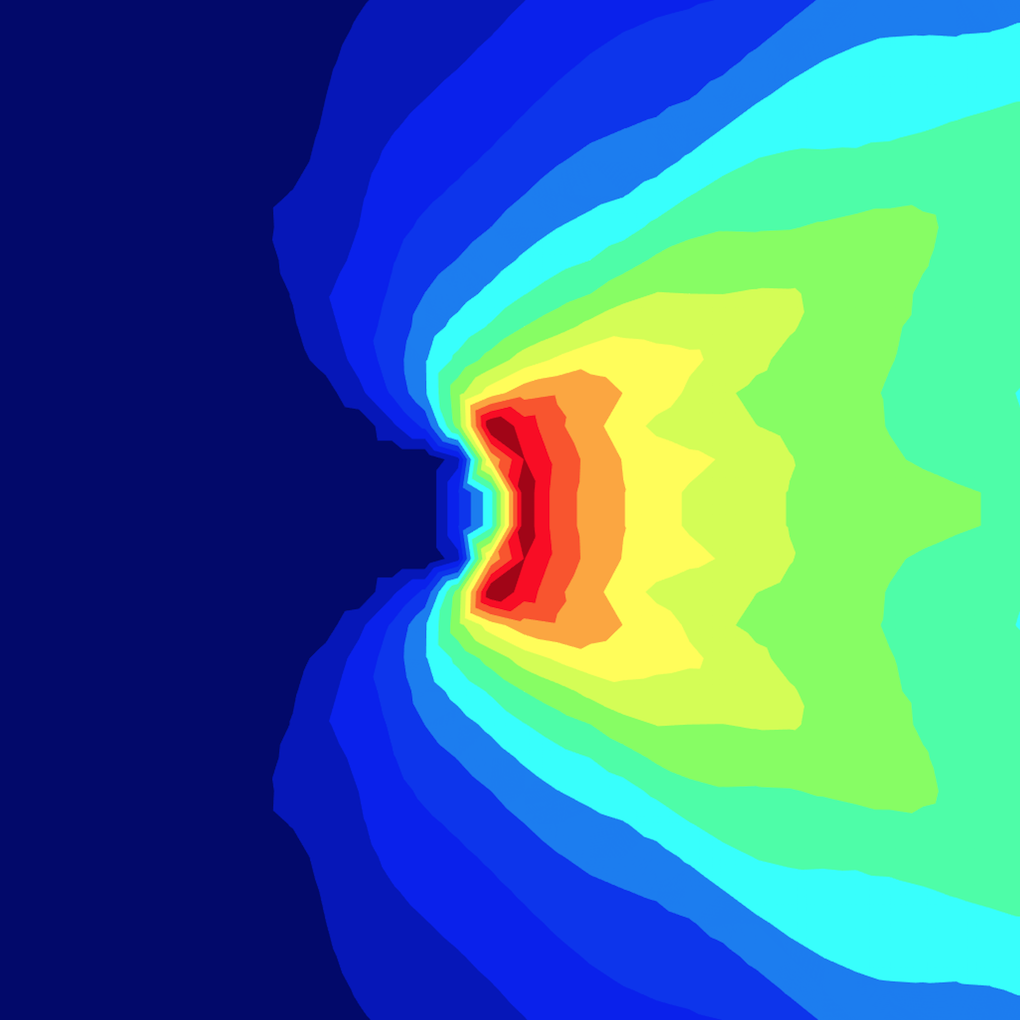
\includegraphics[scale=0.2]{archivos/390} \\
$Dist=3m \; ; \; \phi=30º$  & $Dist=3m \; ; \; \phi=60º$  & $Dist=3m \; ; \; \phi=90º$ \\
\end{tabular}
\caption{Esta es una tabla con múltiples imágenes. Útil cuando se deben mostrar varias juntas.}
\label{multiimagen} % 
\end{table}

Existe también la posibilidad de realizarlo sin tablas, con subfiguras:
\begin{lstlisting}[style=Latex-color]
\begin{figure}[h]
    \centering
    \begin{subfigure}[b]{0.4\textwidth} % Espacio horizontal ocupado por la subfigura
    	\centering
        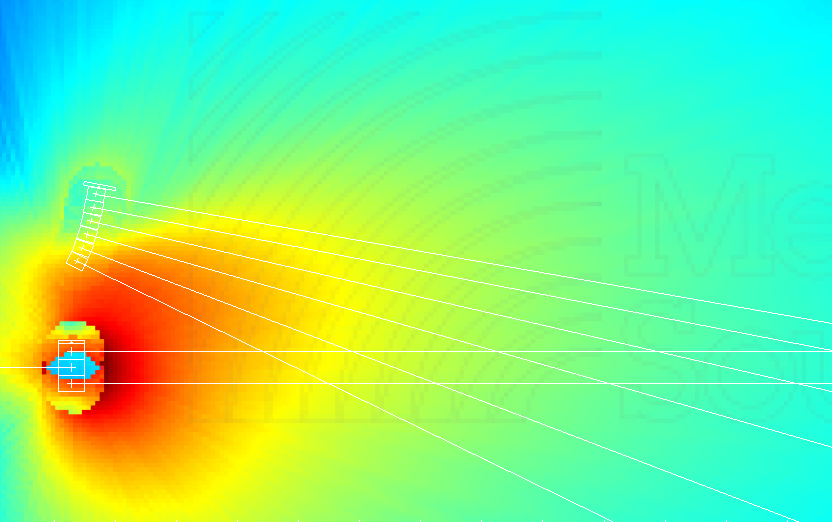
\includegraphics[width=4cm]{archivos/subs-sin} % Tamaño de la imagen
        \caption{Sin procesado.}
        \label{fig:gull}
    \end{subfigure}
    ~ % Añadir el espacio deseado, si se deja la linea en blanco la siguiente subfigura ira en una nueva linea
    \begin{subfigure}[b]{0.4\textwidth} % Espacio horizontal ocupado por la subfigura
    	\centering
        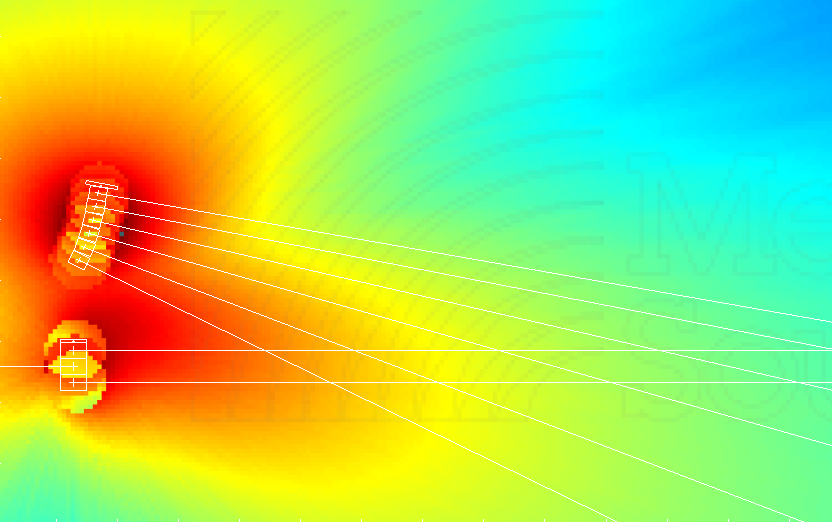
\includegraphics[width=4cm]{archivos/subs-con} % Tamaño de la imagen
        \caption{Con procesado.}
        \label{fig:tiger}
    \end{subfigure}
    \caption{Ejemplo de subfiguras}\label{sistemass}
\end{figure}
\end{lstlisting}
\begin{figure}[h]
    \centering
    \begin{subfigure}[b]{0.4\textwidth}
    	\centering
        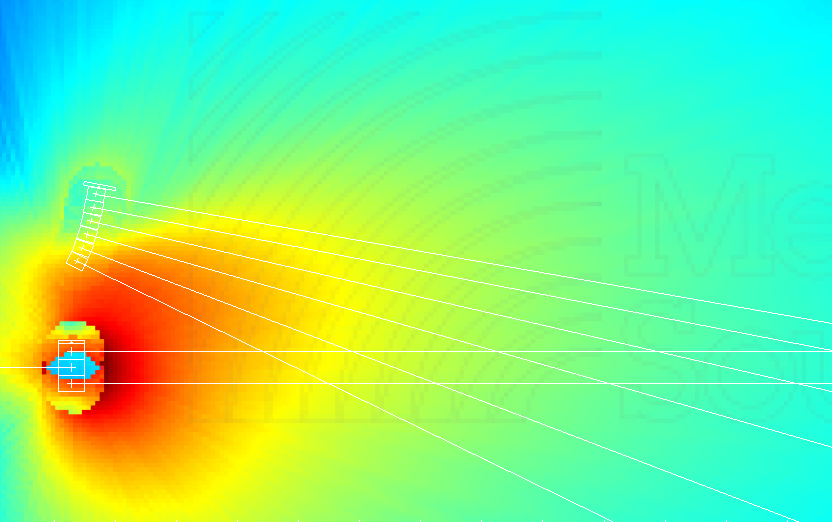
\includegraphics[width=4cm]{archivos/subs-sin}
        \caption{Sin procesado.}
        \label{fig:gull1}
    \end{subfigure}
    ~ % Añadir el espacio deseado, si se deja la linea en blanco la siguiente subfigura ira en una nueva linea
    \begin{subfigure}[b]{0.4\textwidth}
    	\centering
        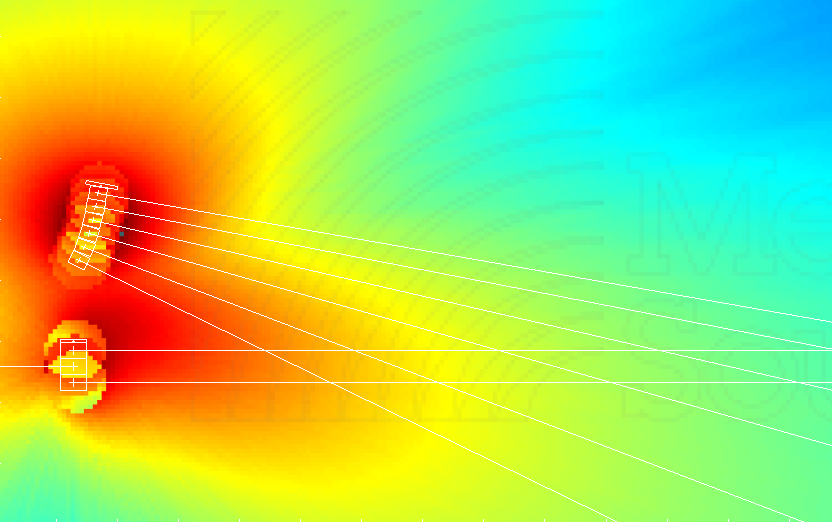
\includegraphics[width=4cm]{archivos/subs-con}
        \caption{Con procesado.}
        \label{fig:tiger1}
    \end{subfigure}
    \caption{Ejemplo de subfiguras}\label{sistemass1}
\end{figure}

\begin{figure}[h]
    \centering
    \begin{subfigure}[b]{\textwidth}
    	\centering
        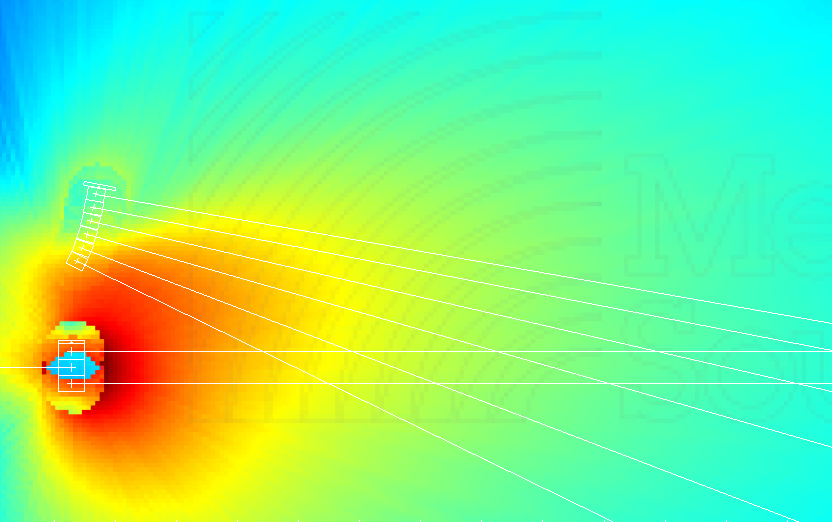
\includegraphics[width=4cm]{archivos/subs-sin}
        \caption{Sin procesado.}
        \label{fig:gull2}
    \end{subfigure}
    
    \begin{subfigure}[b]{\textwidth}
    	\centering
        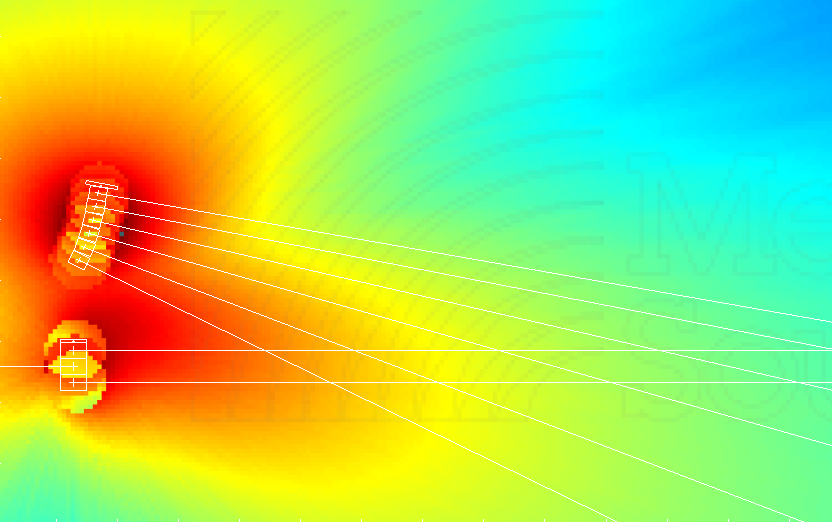
\includegraphics[width=4cm]{archivos/subs-con}
        \caption{Con procesado.}
        \label{fig:tiger2}
    \end{subfigure}
    \caption{Ejemplo de subfiguras vertical}\label{sistemass2}
\end{figure}

Si eliminas la línea '\textbackslash caption' de las subfiguras, tendrás las imágenes sin la información individual, aunque sí con la principal. Y obviamente, si eliminas el de la figura no se mostrará ninguna información.